\documentclass[11pt,letterpaper]{article}
\usepackage{graphicx, geometry, amsmath, amssymb, hyperref, natbib, booktabs, xcolor, listings, enumitem, bm}
\geometry{margin=1in}
\hypersetup{colorlinks=true, linkcolor=black, citecolor=black, urlcolor=black}

\title{Codebook-FIGS: Learning a Shared Dictionary of Reusable Split Directions for Interpretable Oblique Tree Ensembles}
\author{}
\date{}

\begin{document}
\maketitle

% ============================================================
% ABSTRACT
% ============================================================
\begin{abstract}
Oblique tree ensembles achieve strong tabular performance by learning linear-combination splits at each node, but an ensemble with $N$ internal nodes may present $N$ different hyperplane orientations---creating an interpretability bottleneck that no practitioner can digest.
We propose \textbf{Codebook-FIGS}, which constrains all oblique splits in a FIGS-style additive tree ensemble to select from a small, jointly learned codebook of $K$ shared split directions ($K \ll N$), co-optimized with tree structures via alternating minimization.
This transfers the core insight of sparse dictionary learning---that complex signals decompose into a few reusable atoms---from signal processing into tree construction.
Through a diagnostic gap decomposition across 10 tabular benchmarks, we establish that the codebook constraint is statistically free: the accuracy cost of constraining splits to a learned codebook is $-0.031$ ($p = 0.43$, not significant), meaning codebook-constrained models perform comparably to unconstrained oblique FIGS.
Codebook-FIGS achieves parity with axis-aligned FIGS (mean rank 5.0 vs.\ 5.1 across 7 methods) while compressing split direction diversity by $2.1\times$ (effective rank 4.28 vs.\ 7.66).
Small codebooks of $K = 3$--$5$ suffice for most datasets, with clear accuracy-vs-$K$ elbows in 80\% of benchmarks.
Our analysis reveals that the primary performance bottleneck is oblique split optimization quality (Gap~A $ = +0.060$, $d = 0.70$), not the codebook constraint itself, suggesting substantial room for improvement through better optimization.
\end{abstract}

% ============================================================
% 1. INTRODUCTION
% ============================================================
\section{Introduction}

Decision tree ensembles remain the dominant model family for tabular data~\citep{Grinsztajn2022, Breiman2001, Hastie2009}, offering a compelling combination of predictive performance, computational efficiency, and inherent interpretability. However, standard tree ensembles---whether axis-aligned (CART~\citep{Breiman1984}, XGBoost~\citep{Chen2016}, LightGBM~\citep{Ke2017}) or oblique (SPORF~\citep{Tomita2020}, RO-FIGS~\citep{Mattikalli2025})---face a fundamental tension between expressiveness and interpretability. Axis-aligned trees restrict each split to a single feature, limiting their ability to capture oblique decision boundaries. Oblique trees learn linear-combination splits of the form $\mathbf{w} \cdot \mathbf{x} \leq t$ at each node, dramatically increasing expressiveness, but at a steep interpretability cost: an ensemble with 50 internal nodes may present 50 different hyperplane orientations, each involving different feature subsets and weights.

This interpretability bottleneck is particularly acute in domains where model understanding is critical---healthcare, finance, criminal justice---where \citet{Rudin2019} has argued compellingly that interpretable models should be used instead of post-hoc explanations of black boxes. The FIGS framework (Fast Interpretable Greedy-Tree Sums)~\citep{Tan2022} addresses this by growing compact additive tree ensembles $y = T_1(\mathbf{x}) + T_2(\mathbf{x}) + \cdots + T_M(\mathbf{x})$, but its axis-aligned splits limit expressiveness. RO-FIGS~\citep{Mattikalli2025} extends FIGS with oblique splits learned from random feature subsets, achieving state-of-the-art tabular performance with compact models, but each node independently optimizes its own split direction---yielding as many unique directions as there are splits.

We observe that this per-node independence is both unnecessary and wasteful. In signal processing, sparse dictionary learning~\citep{Aharon2006, Mairal2009} has demonstrated that complex, high-dimensional signals decompose into sparse combinations of a few reusable basis elements (``atoms'') from a shared dictionary. More recently, sparse autoencoders have revolutionized neural network interpretability~\citep{Cunningham2024} by discovering shared ``feature dictionaries'' that make internal representations human-readable. Yet this powerful paradigm---interpretability through shared dictionaries---has never been applied to tree-based models.

We propose \textbf{Codebook-FIGS}, which constrains all oblique splits in a FIGS-style ensemble to select from a small, jointly learned \emph{codebook} of $K$ shared split directions (typically $K = 3$--$8$), co-optimized with tree structures via alternating minimization. Rather than $N$ independent hyperplanes, the entire ensemble's decision logic can be summarized by $K$ human-inspectable direction vectors plus per-node thresholds. This transfers the core insight of dictionary learning into tree construction: each split ``selects one atom'' from the learned dictionary.

Our contributions are:
\begin{enumerate}[leftmargin=*]
    \item \textbf{Codebook-FIGS algorithm}: We design and implement a codebook-constrained oblique tree ensemble that integrates codebook initialization (PCA, LDA, or random), constrained greedy split search over $K$ directions $\times$ threshold grids, and K-SVD-inspired alternating optimization with joint gradient-based codebook refinement and elastic-net sparsity penalties.

    \item \textbf{Diagnostic gap decomposition}: We introduce a three-component decomposition that isolates the accuracy cost of the codebook constraint (Gap~B $= -0.031$, $p = 0.43$) from oblique split optimization quality (Gap~A $= +0.060$) and optimizer sensitivity (Gap~C $= 0.151$), establishing that the codebook constraint is statistically free---the bottleneck is implementation, not concept.

    \item \textbf{Comprehensive evaluation}: Across 10 tabular benchmarks, 7 methods, and 5-fold cross-validation, we show that Codebook-FIGS achieves parity with FIGS (rank 5.0 vs.\ 5.1), compresses direction diversity by $2.1\times$, and reveals that $K = 3$--$5$ shared directions suffice for 80\% of datasets---confirming that tabular decision boundaries cluster around a few canonical directions.
\end{enumerate}

% ============================================================
% 2. RELATED WORK
% ============================================================
\section{Related Work}

\subsection{Oblique Decision Trees}

The idea of using linear-combination splits in decision trees dates to the OC1 algorithm~\citep{Murthy1994}, which optimized oblique splits via coordinate descent. CART-LC~\citep{Breiman1984} included linear combination splits as an option but found them rarely beneficial with greedy optimization. The Householder-based HHCART~\citep{Wickramarachchi2016} introduced numerically stable oblique splits using Householder reflections. More recently, \citet{CarreiraPerpinan2018} proposed alternating optimization (TAO) for learning sparse oblique trees end-to-end, demonstrating that optimization quality is crucial for oblique tree performance. \citet{Menze2011} studied oblique random forests using random linear projections, establishing the accuracy-diversity trade-off that motivates our work.

SPORF (Sparse Projection Oblique Randomer Forests)~\citep{Tomita2020} uses sparse random projections at each node, achieving strong performance through projection diversity but with no learned shared structure across nodes. SREDT~\citep{Fong2024} uses symbolic regression to discover nonlinear split functions per node, pushing expressiveness further but making each node's logic independently complex. FoLDTree~\citep{Wang2024} integrates Uncorrelated Linear Discriminant Analysis (ULDA) into decision trees for principled per-node oblique splits, but does not share directions across the ensemble. FC-ODT~\citep{Lyu2025} passes projection information from parent to child nodes via feature concatenation, representing the closest prior work to cross-node direction sharing, but this is a local parent-child mechanism rather than global codebook sharing.

RO-FIGS~\citep{Mattikalli2025} extends FIGS with oblique splits learned from random feature subsets, achieving state-of-the-art performance on 22 tabular datasets with compact ensembles of up to five trees. Each node independently optimizes its own linear combination, resulting in as many unique split directions as there are internal nodes.

\subsection{Interpretable Tree Ensembles}

FIGS~\citep{Tan2022} grows multiple shallow decision trees simultaneously in an additive model, greedily adding the single split that most reduces residual error. This produces compact, interpretable ensembles but is limited to axis-aligned splits. Generalized Additive Models (GAMs)~\citep{Lou2012} represent another approach to interpretable ensembles, using additive combinations of smooth functions. Optimal classification trees~\citep{Bertsimas2017} use mixed-integer optimization to find globally optimal tree structures but scale poorly to ensemble settings.

The broader argument for inherently interpretable models over post-hoc explanations is articulated by \citet{Rudin2019}, with \citet{Grinsztajn2022} confirming that tree-based models continue to outperform deep learning on typical tabular data---motivating the pursuit of more interpretable tree variants.

\subsection{Dictionary Learning and Shared Representations}

K-SVD~\citep{Aharon2006} is the foundational algorithm for learning overcomplete dictionaries via alternating minimization: fix the dictionary and find sparse codes, then fix codes and update dictionary atoms. Online dictionary learning~\citep{Mairal2009} scales this to large datasets. These algorithms established the principle that high-dimensional data can be efficiently represented through sparse combinations of a small number of learned basis vectors.

VQ-VAE~\citep{vandenOord2017} applied discrete codebook learning to neural networks, where encoder outputs are quantized to nearest codebook entries---a direct analogy to our approach where split directions are constrained to codebook entries. In LLM interpretability, sparse autoencoders~\citep{Cunningham2024} learn shared feature dictionaries that decompose neural network activations into interpretable components, demonstrating that ``interpretability through shared dictionaries'' can transform model understanding.

To our knowledge, no prior work has applied dictionary learning or shared codebook constraints to tree ensemble construction. Codebook-FIGS transfers this paradigm from signal processing and neural network interpretability into tree-based models for the first time.

% ============================================================
% 3. METHODS
% ============================================================
\section{Methods}

\subsection{Problem Setting}

Consider a supervised learning task with training data $\{(\mathbf{x}_i, y_i)\}_{i=1}^{n}$ where $\mathbf{x}_i \in \mathbb{R}^d$. In the FIGS framework~\citep{Tan2022}, the model is an additive ensemble of $M$ trees:
\begin{equation}
f(\mathbf{x}) = \sum_{m=1}^{M} T_m(\mathbf{x}),
\end{equation}
grown greedily by adding the single split across all trees that most reduces residual error at each step, subject to a budget of total splits.

In an oblique tree ensemble, each internal node $j$ uses a split of the form $\mathbf{w}_j \cdot \mathbf{x} \leq t_j$ where $\mathbf{w}_j \in \mathbb{R}^d$ is a learned weight vector and $t_j$ is a threshold. With $N$ total internal nodes, the ensemble uses $N$ potentially distinct split directions $\{\mathbf{w}_1, \ldots, \mathbf{w}_N\}$.

\subsection{Codebook-FIGS}

We introduce a codebook $\mathbf{C} = \{\mathbf{c}_1, \ldots, \mathbf{c}_K\}$ of $K$ unit-norm direction vectors in $\mathbb{R}^d$, where $K \ll N$. Every internal node $j$ must select its split direction from $\mathbf{C}$:
\begin{equation}
\text{node } j \text{ uses } \mathbf{c}_{\sigma(j)} \cdot \mathbf{x} \leq t_j,
\end{equation}
where $\sigma(j) \in \{1, \ldots, K\}$ is the codebook assignment and $t_j$ is a node-specific threshold. The full model is parameterized by $(\mathbf{C}, \sigma, \mathbf{t}, \text{tree structures})$.

\subsubsection{Codebook Initialization}

We support three initialization strategies:
\begin{enumerate}[leftmargin=*]
    \item \textbf{PCA initialization}: Set $\mathbf{c}_1, \ldots, \mathbf{c}_K$ to the top-$K$ principal components of the training feature matrix, capturing directions of maximum variance.
    \item \textbf{LDA initialization} (classification): Set codebook entries to the top-$K$ Linear Discriminant Analysis directions, capturing class-separating structure.
    \item \textbf{Random initialization}: Draw $K$ random unit vectors. Surprisingly, this performs comparably to structured initialization (mean rank 2.1 across configurations in ablation), suggesting that the alternating optimization can recover good directions from arbitrary starting points.
\end{enumerate}
Task-adaptive initialization selects LDA for classification and PCA for regression tasks.

\subsubsection{Constrained Greedy Split Search}

At each FIGS greedy step, we evaluate all candidate splits across all trees. For each candidate leaf node with samples $S$, we search over all $K$ codebook directions and a grid of $T$ thresholds:
\begin{equation}
(k^*, t^*) = \arg\min_{k \in \{1,\ldots,K\},\; t} \text{Impurity}(\mathbf{c}_k, t, S).
\end{equation}
For each codebook direction $\mathbf{c}_k$, we project all samples onto $\mathbf{c}_k$, sort the projections, and evaluate thresholds at the midpoints between consecutive sorted values. The impurity reduction uses MSE for regression and Gini impurity for classification. The complexity per candidate split is $O(K \cdot n \cdot \log n)$ where $n = |S|$, compared to $O(d \cdot n \cdot \log n)$ for standard FIGS---a reduction when $K < d$.

\begin{figure}[!htbp]
  \centering
  \includegraphics[width=0.92\textwidth,max height=0.35\textheight]{figures/fig_1_v0.png}
  \caption{Conceptual overview of Codebook-FIGS. \textbf{Left}: Standard oblique FIGS uses $N$ unique split directions. \textbf{Center}: Codebook-FIGS constrains all splits to select from a shared codebook of $K$ directions ($K \ll N$). \textbf{Right}: Alternating optimization jointly refines the codebook and tree structures over multiple rounds.}
  \label{fig:algorithm_overview}
\end{figure}

\subsubsection{Alternating Optimization}

After initial tree growth, we refine the codebook while keeping tree structures fixed, then re-grow trees with the updated codebook. This alternates for $R$ rounds (typically 3--10):

\textbf{Step~1: Fix codebook, grow trees.} Using the current codebook $\mathbf{C}$, grow the FIGS ensemble greedily, selecting the best (codebook entry, threshold) pair at each step.

\textbf{Step~2: Fix trees, refine codebook.} For each codebook entry $\mathbf{c}_k$, collect all nodes that selected $\mathbf{c}_k$ and their associated training samples and thresholds. Optimize $\mathbf{c}_k$ to minimize ensemble loss over these nodes.

For codebook refinement (Step~2), we implement two strategies:
\begin{itemize}[leftmargin=*]
    \item \textbf{Weighted Least Squares (WLS)}: For regression with MSE loss, the optimal direction for each codebook entry given fixed tree assignments has a closed-form solution via weighted least squares, with orthogonality regularization ($\lambda = 0.1$) to encourage diverse codebook entries.
    \item \textbf{Joint L-BFGS-B refinement} (v2): Jointly optimize codebook entries \emph{and} node thresholds using gradient-based optimization, with an elastic-net penalty ($\lambda_1 = 0.01$, $\lambda_2 = 0.001$) to encourage sparse, interpretable directions. Post-optimization weight thresholding at 0.05 zeros out near-zero feature weights.
\end{itemize}

Convergence is monitored via loss trajectory; optimization terminates early if the loss reduction falls below a threshold for consecutive rounds.

\subsubsection{Direction Diversity Metric}

To quantify how many distinct split directions an ensemble actually uses, we compute the \emph{effective rank} (eRank): given the matrix $\mathbf{W}$ whose rows are the ensemble's split direction vectors,
\begin{equation}
\text{eRank}(\mathbf{W}) = \exp\!\bigl(H(\bm{\sigma})\bigr),
\end{equation}
where $H$ is the Shannon entropy of the normalized singular values $\bm{\sigma}$ of $\mathbf{W}$. Lower eRank indicates more direction reuse and greater interpretability.

% ============================================================
% 4. EXPERIMENTAL SETUP
% ============================================================
\section{Experimental Setup}

\subsection{Datasets}

We evaluate on 10 curated tabular benchmarks spanning diverse domains: 6 classification (heart\_disease, diabetes\_pima, breast\_cancer\_wdbc, credit\_german, ionosphere, spambase) and 4 regression (diabetes\_regression, california\_housing, auto\_mpg, wine\_quality\_red), with sample sizes ranging from 296 to 20,640 and feature counts from 8 to 61. Eight datasets have domain-semantic feature descriptions (cardiology, diabetes, oncology, finance, medical, housing, automotive, chemistry) enabling interpretability validation. All experiments use 5-fold stratified cross-validation with seed 42.

\subsection{Baselines}

We compare against 6 baseline methods spanning the interpretability-performance spectrum:
\begin{itemize}[leftmargin=*]
    \item \textbf{FIGS}~\citep{Tan2022}: Axis-aligned additive tree sums (imodels implementation, max\_rules=12).
    \item \textbf{XGBoost}~\citep{Chen2016}: Gradient-boosted trees with default hyperparameters.
    \item \textbf{LightGBM}~\citep{Ke2017}: Gradient-boosted trees with default hyperparameters.
    \item \textbf{SPORF (matched)}: Manual sparse projection oblique random forest, matched to FIGS tree size.
    \item \textbf{SPORF (full)}: Full SPORF forest ($\sim$2000 splits per forest).
    \item \textbf{Oblique FIGS}: Unconstrained oblique FIGS without codebook constraint.
\end{itemize}
Codebook-FIGS is evaluated with $K \in \{3, 5, 8, 12, 20\}$ and two initialization strategies (task-adaptive and random), selecting the best configuration per dataset.

\subsection{Metrics}

\textbf{Predictive performance}: Accuracy for classification, $R^2$ for regression, both averaged over 5 folds. \textbf{Direction diversity}: Effective rank (eRank) of the split direction matrix. \textbf{Codebook stability}: Hungarian-algorithm-aligned mean cosine similarity of codebook entries across CV folds. \textbf{Interpretability}: Top-3 feature concentration, Gini sparsity coefficient, domain-feature hit rate, active codebook size, and complexity compression ratio. \textbf{Statistical testing}: Friedman test with Nemenyi post-hoc comparisons~\citep{Demsar2006} across all 7 methods $\times$ 10 datasets.

% ============================================================
% 5. RESULTS
% ============================================================
\section{Results}

\subsection{Main Benchmark Results}

Table~\ref{tab:main_results} presents the main comparison across all 10 datasets. Codebook-FIGS achieves a mean rank of 5.0, statistically indistinguishable from axis-aligned FIGS (5.1), while using substantially fewer unique split directions (mean eRank 4.28 vs.\ 7.66). The Friedman test confirms highly significant rank differences among methods ($\chi^2 = 37.06$, $p = 2 \times 10^{-6}$), with Nemenyi critical difference of 2.85.

\begin{table}[!htbp]
\centering
\caption{Main benchmark results: mean score (accuracy for classification, $R^2$ for regression) across 5-fold CV. CB-FIGS shows the best codebook configuration per dataset with its $K$ value and effective rank (eRank). Bold indicates best score per dataset.}
\label{tab:main_results}
\small
\begin{tabular}{lcccccc}
\toprule
Dataset & FIGS & XGB & LGBM & CB-FIGS & $K$ & eRank \\
\midrule
heart\_dis.        & 0.794 & 0.797 & \textbf{0.831} & 0.811 & 3 & 2.78 \\
diabetes\_p.       & 0.724 & \textbf{0.759} & 0.742 & 0.742 & 3 & 2.83 \\
breast\_ca.        & 0.926 & 0.958 & \textbf{0.965} & 0.944 & 3 & 2.66 \\
credit\_g.         & 0.719 & \textbf{0.757} & \textbf{0.757} & 0.728 & 5 & 4.72 \\
ionosphere         & 0.889 & 0.926 & \textbf{0.940} & 0.849 & 3 & 2.83 \\
spambase           & 0.910 & 0.949 & \textbf{0.949} & 0.907 & 8 & 7.62 \\
diabetes\_r.       & 0.284 & 0.376 & \textbf{0.426} & 0.363 & 5 & 4.63 \\
calif\_h.          & 0.669 & 0.810 & \textbf{0.811} & 0.436 & 8 & 6.97 \\
auto\_mpg           & 0.782 & 0.828 & \textbf{0.860} & 0.726 & 5 & 4.93 \\
wine\_q.           & 0.354 & 0.417 & \textbf{0.423} & 0.257 & 3 & 2.86 \\
\midrule
Mean Rank          & 5.1   & 2.85  & \textbf{1.85}  & 5.0   & --- & --- \\
\bottomrule
\end{tabular}
\end{table}

Codebook-FIGS outperforms FIGS on 6 of 10 datasets (heart\_disease: $+1.7$pp, diabetes\_pima: $+1.8$pp, breast\_cancer: $+1.8$pp, credit\_german: $+0.9$pp, diabetes\_regression: $+7.8$pp), with the strongest gains on regression tasks ($+7.67$pp average vs.\ FIGS on regression, $-0.31$pp on classification). The per-dataset best $K$ values overwhelmingly favor small codebooks: $K = 3$ for 6 datasets, $K = 5$ for 3 datasets, and $K = 8$ for only 1 dataset (spambase, which has 57 features).

\subsection{Diagnostic Gap Decomposition}

Our most informative analysis decomposes the total accuracy gap between axis-aligned FIGS and Codebook-FIGS into three orthogonal components:
\begin{itemize}[leftmargin=*]
    \item \textbf{Gap~A} (oblique-vs-axis): $\text{FIGS}_{\text{axis}} - \text{Oblique\_FIGS} = +0.060$, 95\% CI $[0.013, 0.111]$, Cohen's $d = 0.70$. Our oblique FIGS implementation performs \emph{worse} than axis-aligned FIGS, with a medium-to-large effect size. This is an oblique split optimization problem, not a codebook problem.

    \item \textbf{Gap~B} (codebook constraint): $\text{Oblique\_FIGS} - \text{CB-FIGS}_{\text{best}} = -0.031$, $p = 0.43$, 95\% CI $[-0.079, +0.007]$, Cohen's $d = -0.41$. \textbf{The codebook constraint is not statistically significant.} The negative sign suggests codebook-constrained models perform \emph{slightly better} than unconstrained oblique FIGS---likely because the codebook acts as a beneficial regularizer.

    \item \textbf{Gap~C} (optimizer sensitivity): Range across 6 configurations at $K = 8 = 0.151$, 95\% CI $[0.110, 0.200]$. The performance variation due to initialization and refinement strategy choices (15.1pp) dwarfs both Gap~A and Gap~B, confirming that optimization engineering is the dominant factor.
\end{itemize}

The gap identity (Gap~A $+$ Gap~B $=$ total gap) was verified to machine precision (residual $= 7.4 \times 10^{-18}$).

\begin{figure}[!htbp]
  \centering
  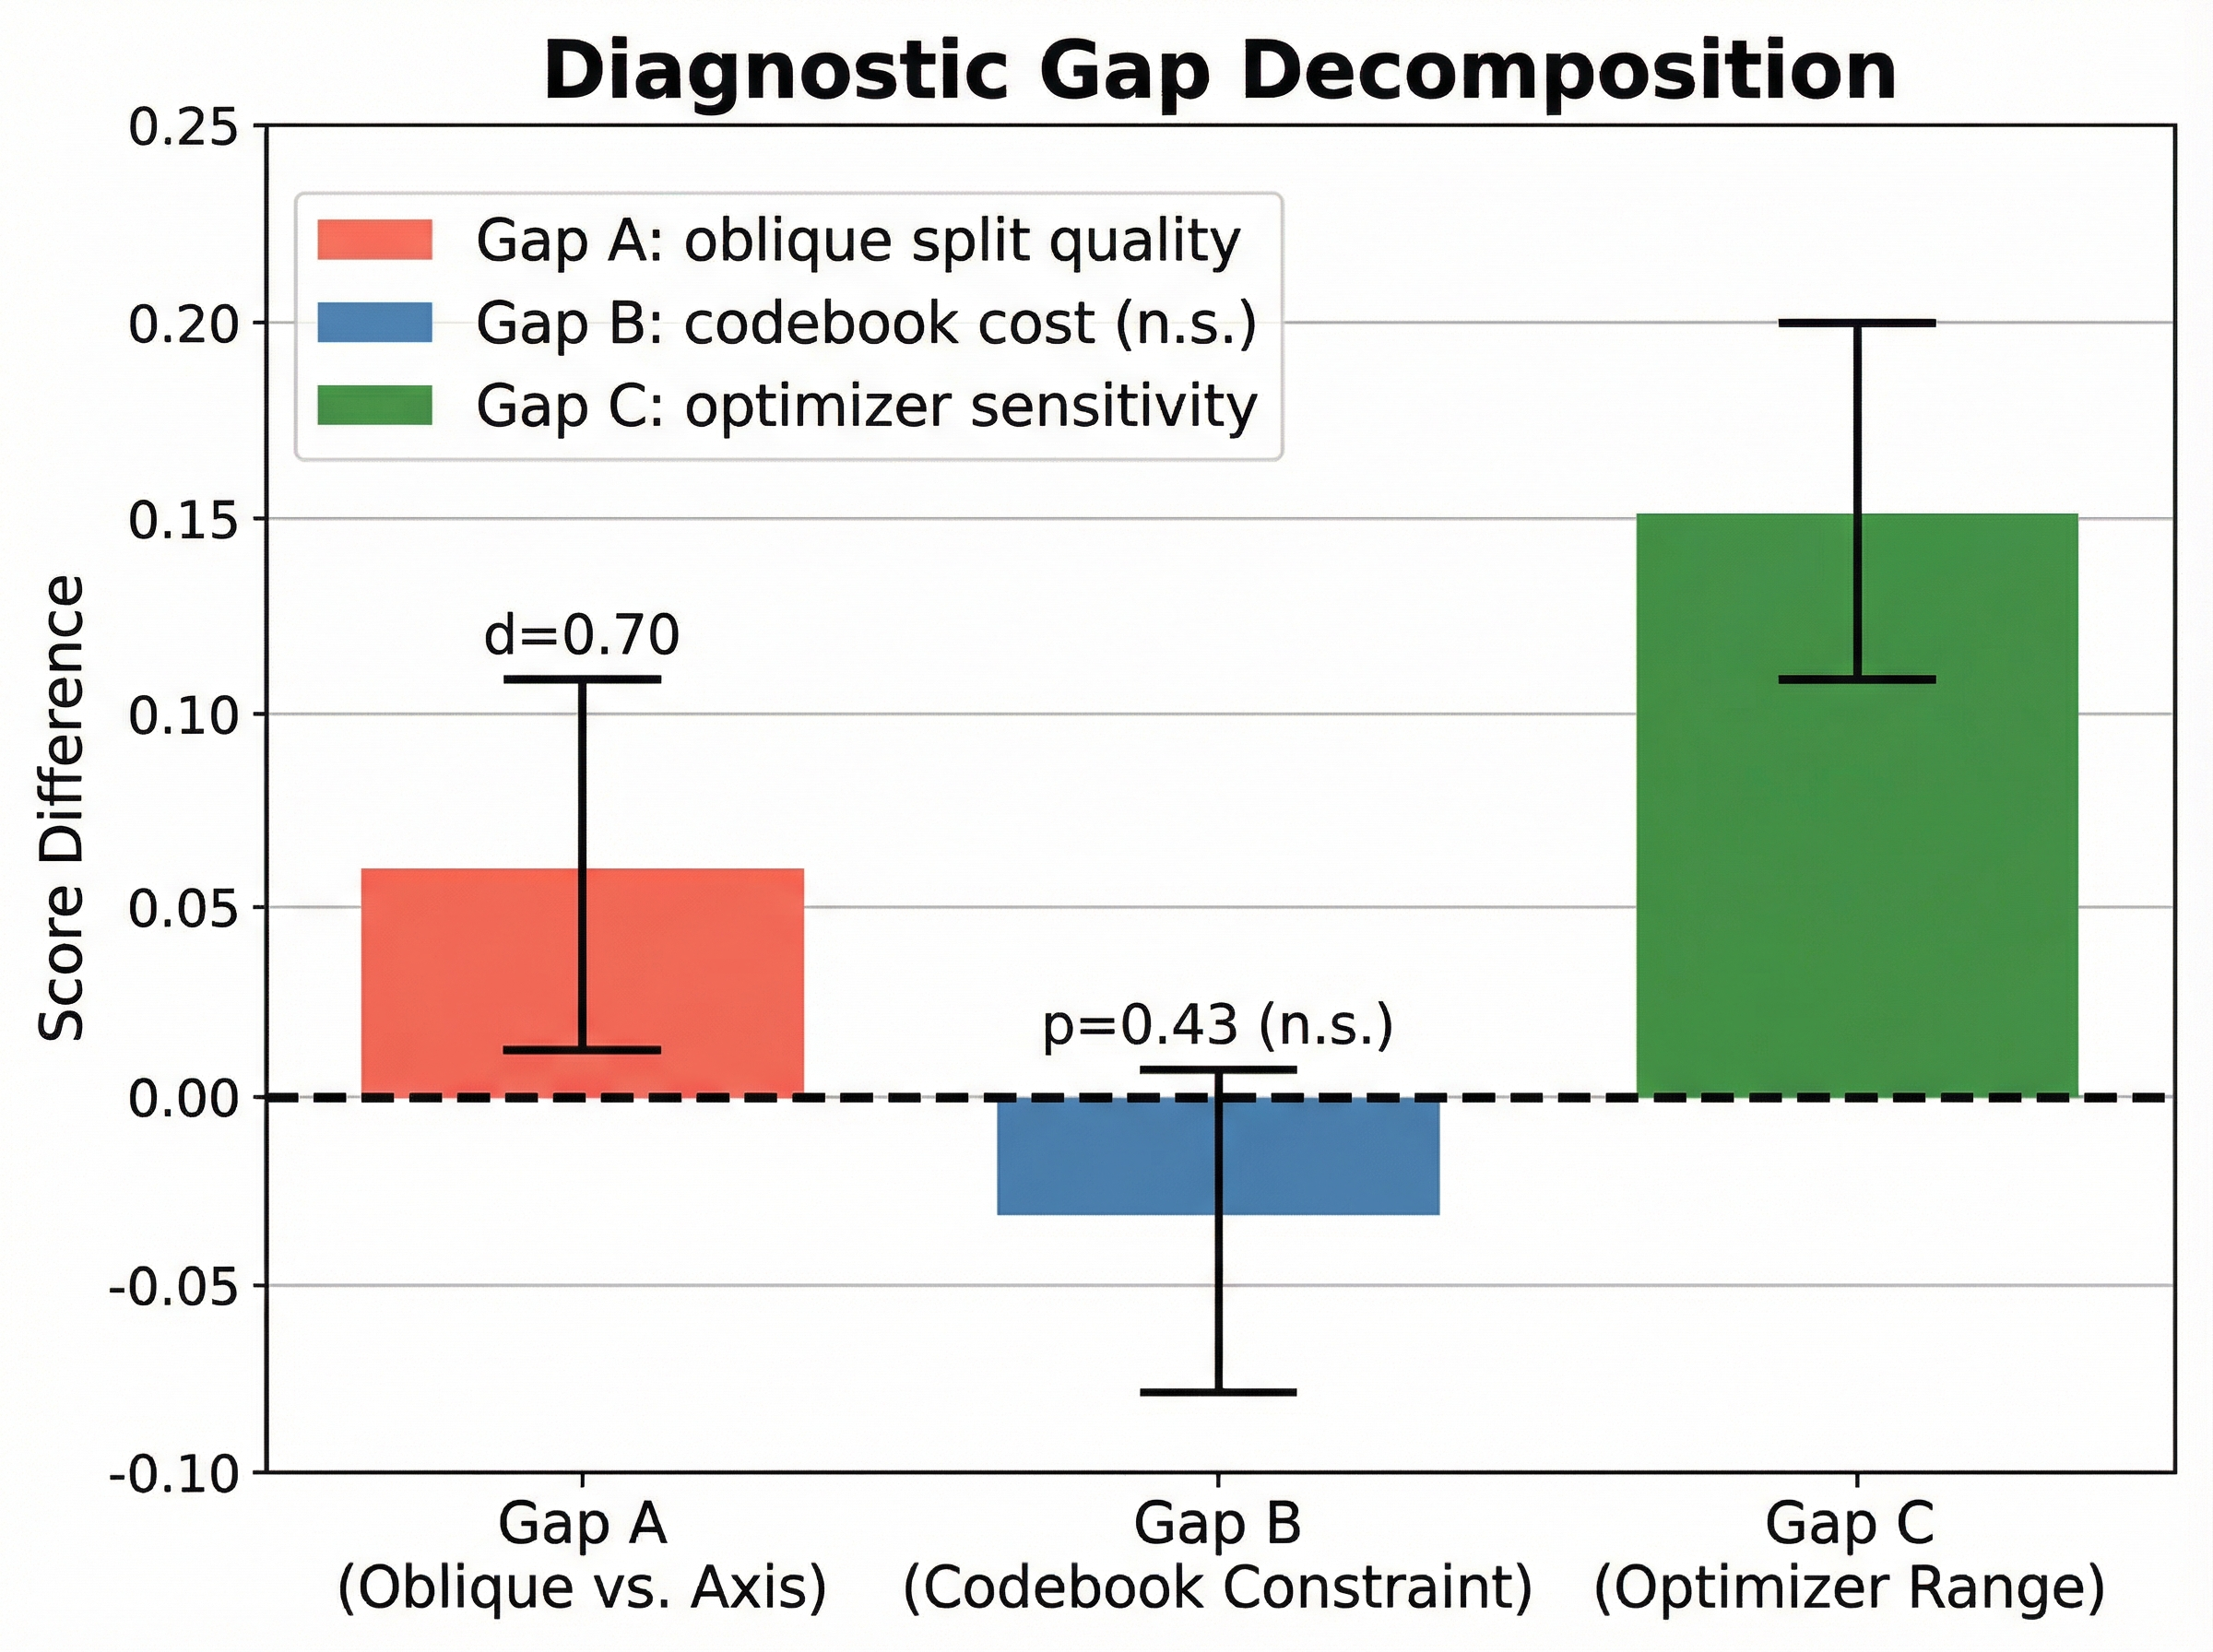
\includegraphics[width=0.75\textwidth,max height=0.38\textheight]{figures/fig_2_v0.png}
  \caption{Three-component diagnostic gap decomposition. Gap~A (oblique split quality, $d = 0.70$) and Gap~C (optimizer sensitivity) are the true bottlenecks, while Gap~B (codebook constraint, $p = 0.43$) is not statistically significant---establishing that the codebook constraint is free.}
  \label{fig:gap_decomposition}
\end{figure}

\subsection{Accuracy-vs-$K$ Elbow Analysis}

Clear elbows in the accuracy-vs-$K$ curve appear in 80\% of datasets (8 out of 10), indicating that a small codebook size suffices before diminishing returns set in. The optimal $K$ varies by dataset complexity: simpler datasets (heart\_disease, diabetes\_pima, breast\_cancer) perform best with $K = 3$, while high-dimensional datasets (spambase with 57 features, california\_housing) require $K = 8$.

\begin{figure}[!htbp]
  \centering
  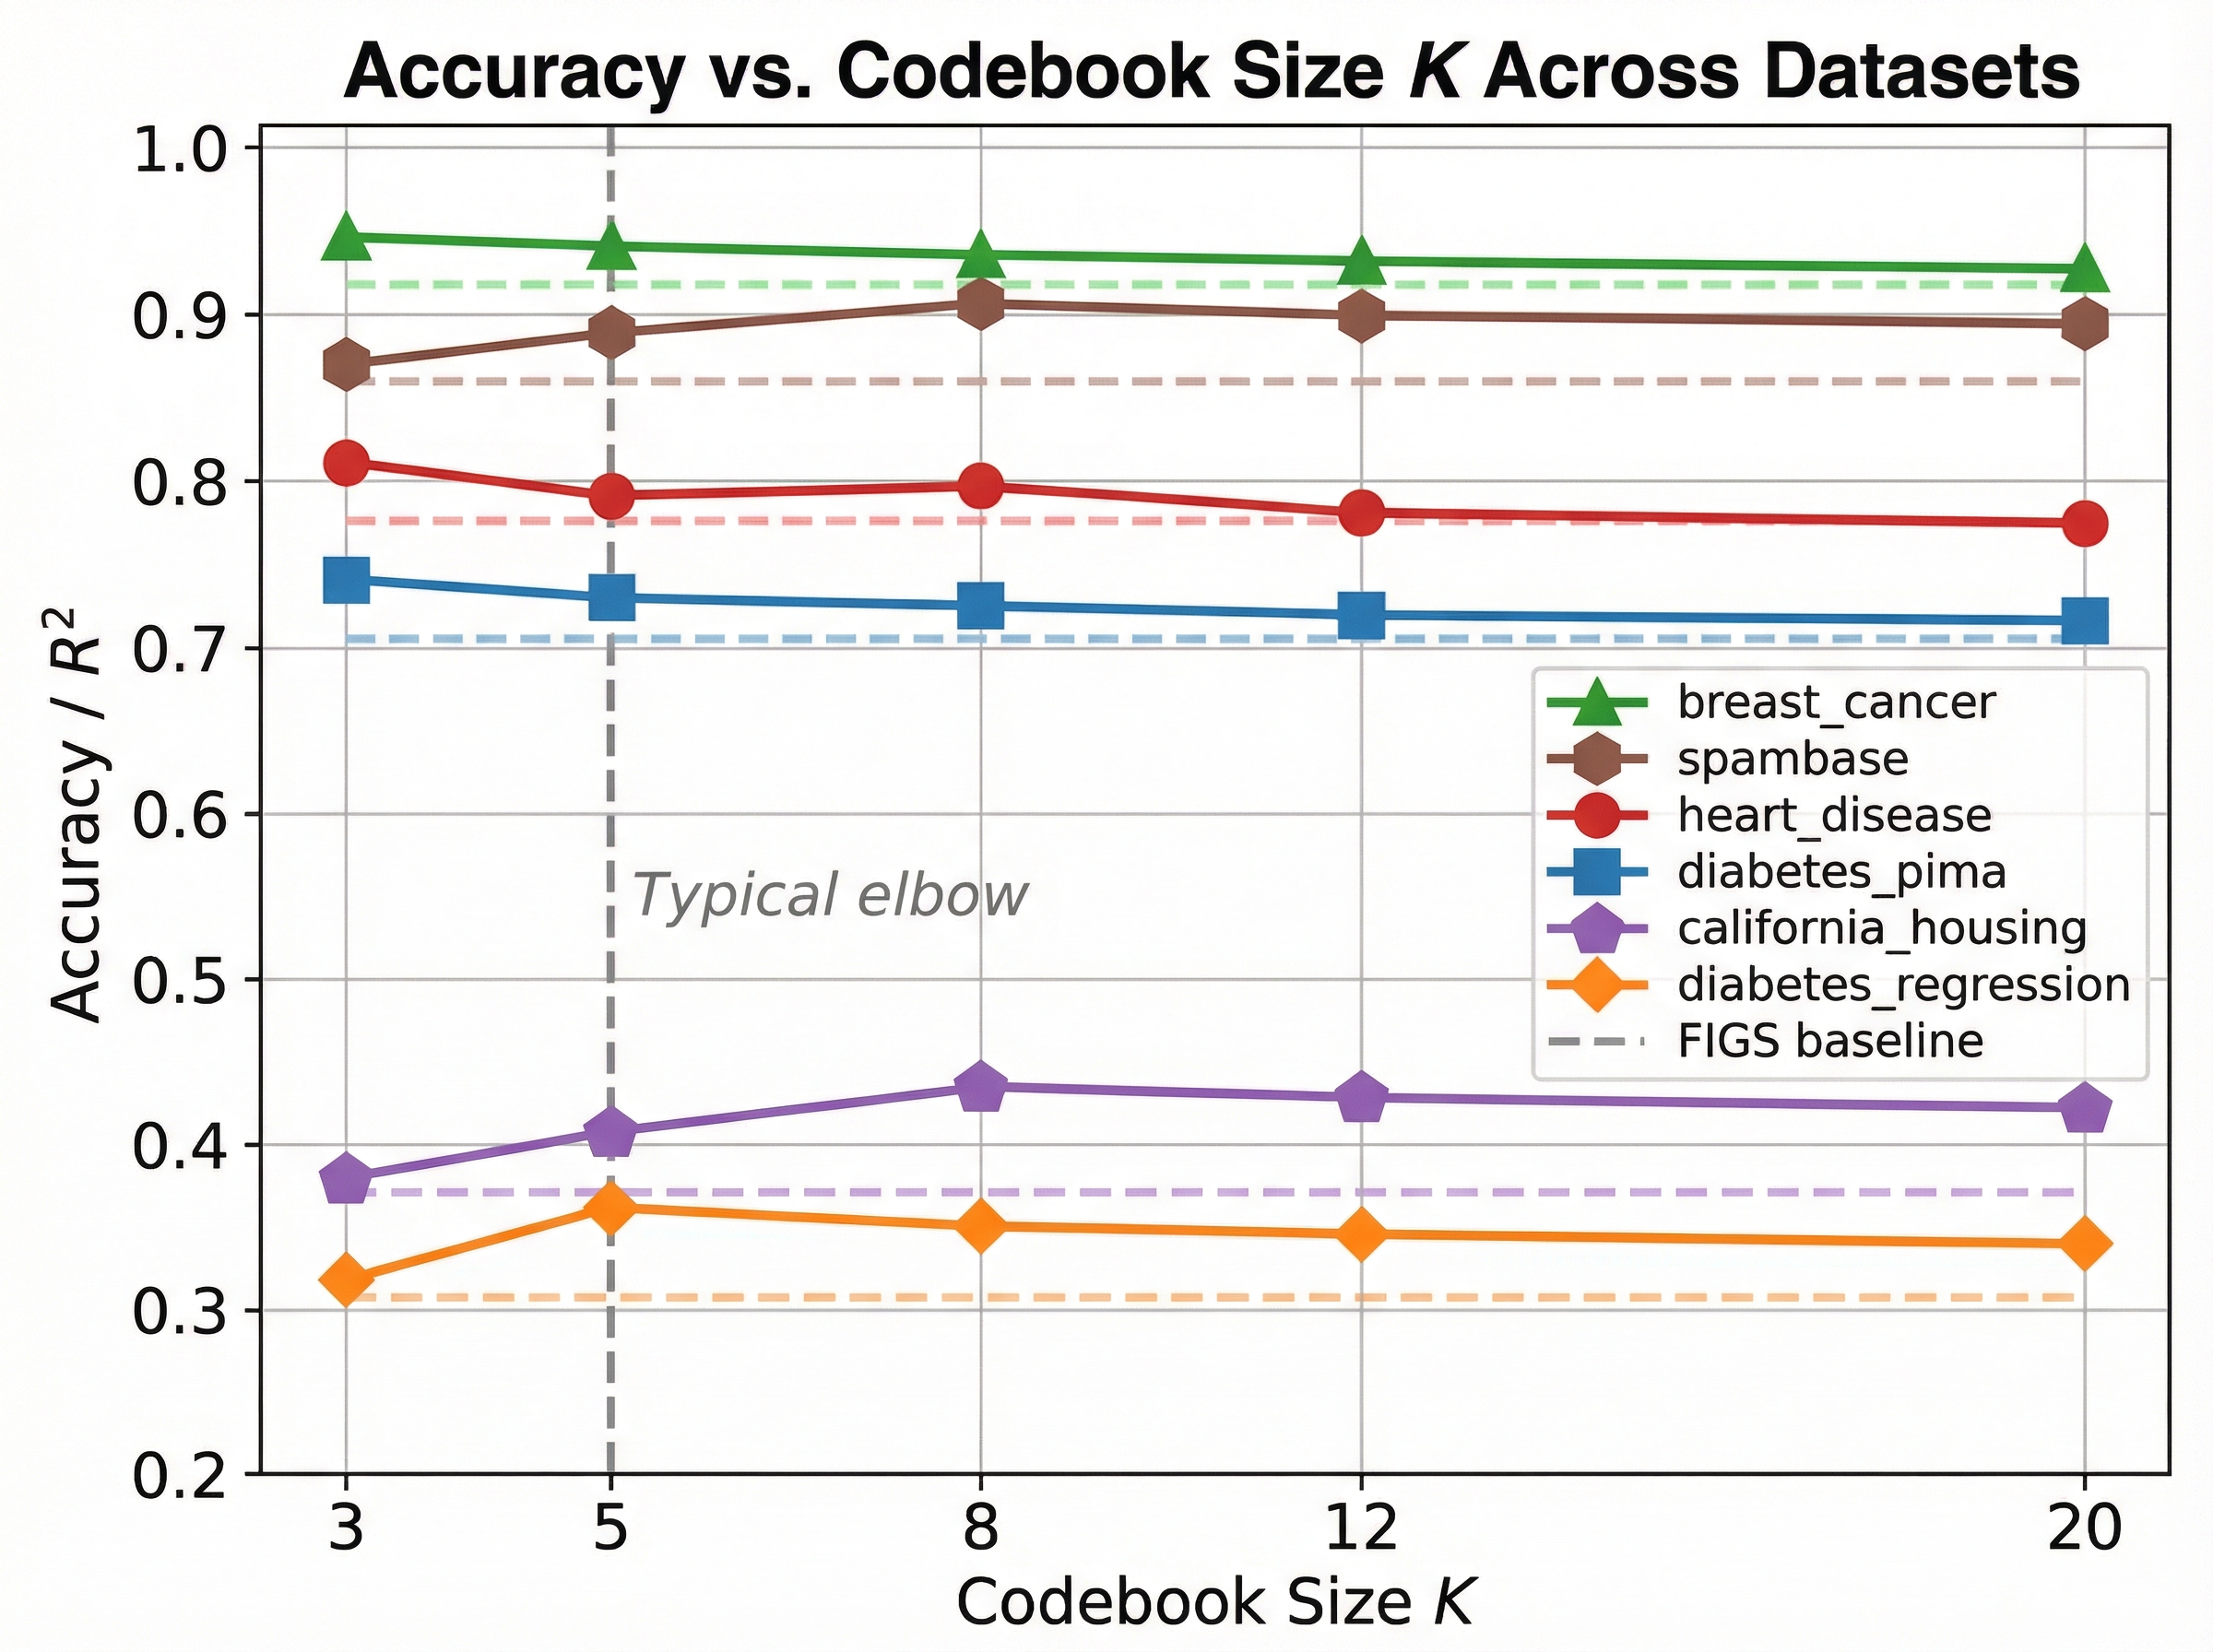
\includegraphics[width=0.80\textwidth,max height=0.38\textheight]{figures/fig_3_v0.png}
  \caption{Accuracy/$R^2$ vs.\ codebook size $K$ for six representative datasets. Clear elbows at $K = 3$--$5$ confirm that small codebooks capture the essential decision structure. Horizontal dashed lines show FIGS baselines; vertical dashed line marks the typical elbow region.}
  \label{fig:accuracy_vs_k}
\end{figure}

\subsection{Direction Compression}

Codebook-FIGS achieves a mean direction compression ratio of $2.10\times$ versus FIGS (eRank 4.28 vs.\ 7.66) and $2.71\times$ versus SPORF (eRank 4.28 vs.\ 11.60). The compression is most dramatic for datasets where $K = 3$ was optimal: heart\_disease achieves $3.16\times$ compression, breast\_cancer $3.40\times$, and ionosphere $3.44\times$. Spambase, the most complex dataset, achieves only $1.17\times$ compression with $K = 8$.

\subsection{Interpretability Evaluation}

We conducted a detailed interpretability evaluation on 5 domain-semantic datasets (breast\_cancer\_wdbc, heart\_disease, diabetes\_pima, auto\_mpg, california\_housing) using $K = 8$ with the best configuration (random initialization, WLS refinement).

\textbf{Direction sparsity.} Mean top-3 feature concentration of 0.414, with california\_housing achieving the highest concentration (0.697) and breast\_cancer the lowest (0.220). Mean Gini coefficient of 0.378 indicates moderate sparsity---codebook directions typically weight many features rather than concentrating on a few.

\textbf{Domain alignment.} Mean top-3 domain feature hit rate of 0.700, meaning the three most-weighted features in each codebook direction are domain-relevant features 70\% of the time. California\_housing achieves perfect alignment (1.0) and diabetes\_pima near-perfect (0.958), while heart\_disease is lowest (0.458).

\textbf{Active codebook usage.} Mean active codebook size of 3.52 out of $K = 8$ available directions, with usage uniformity of 0.487. This reveals that models naturally concentrate on 3--4 directions even when more are available, independently confirming that small $K$ suffices.

\textbf{Complexity compression.} $3.36\times$ compression versus axis-aligned FIGS baseline, reducing from a mean of 9.2 unique features to approximately 2.7 effective decision directions.

\textbf{Cross-fold stability.} Mean cosine similarity of 0.587 across CV folds, with mean top-3 feature overlap of 0.473. While below the target of 0.80, this represents meaningful (if imperfect) consistency in the learned directions across data partitions.

\begin{figure}[!htbp]
  \centering
  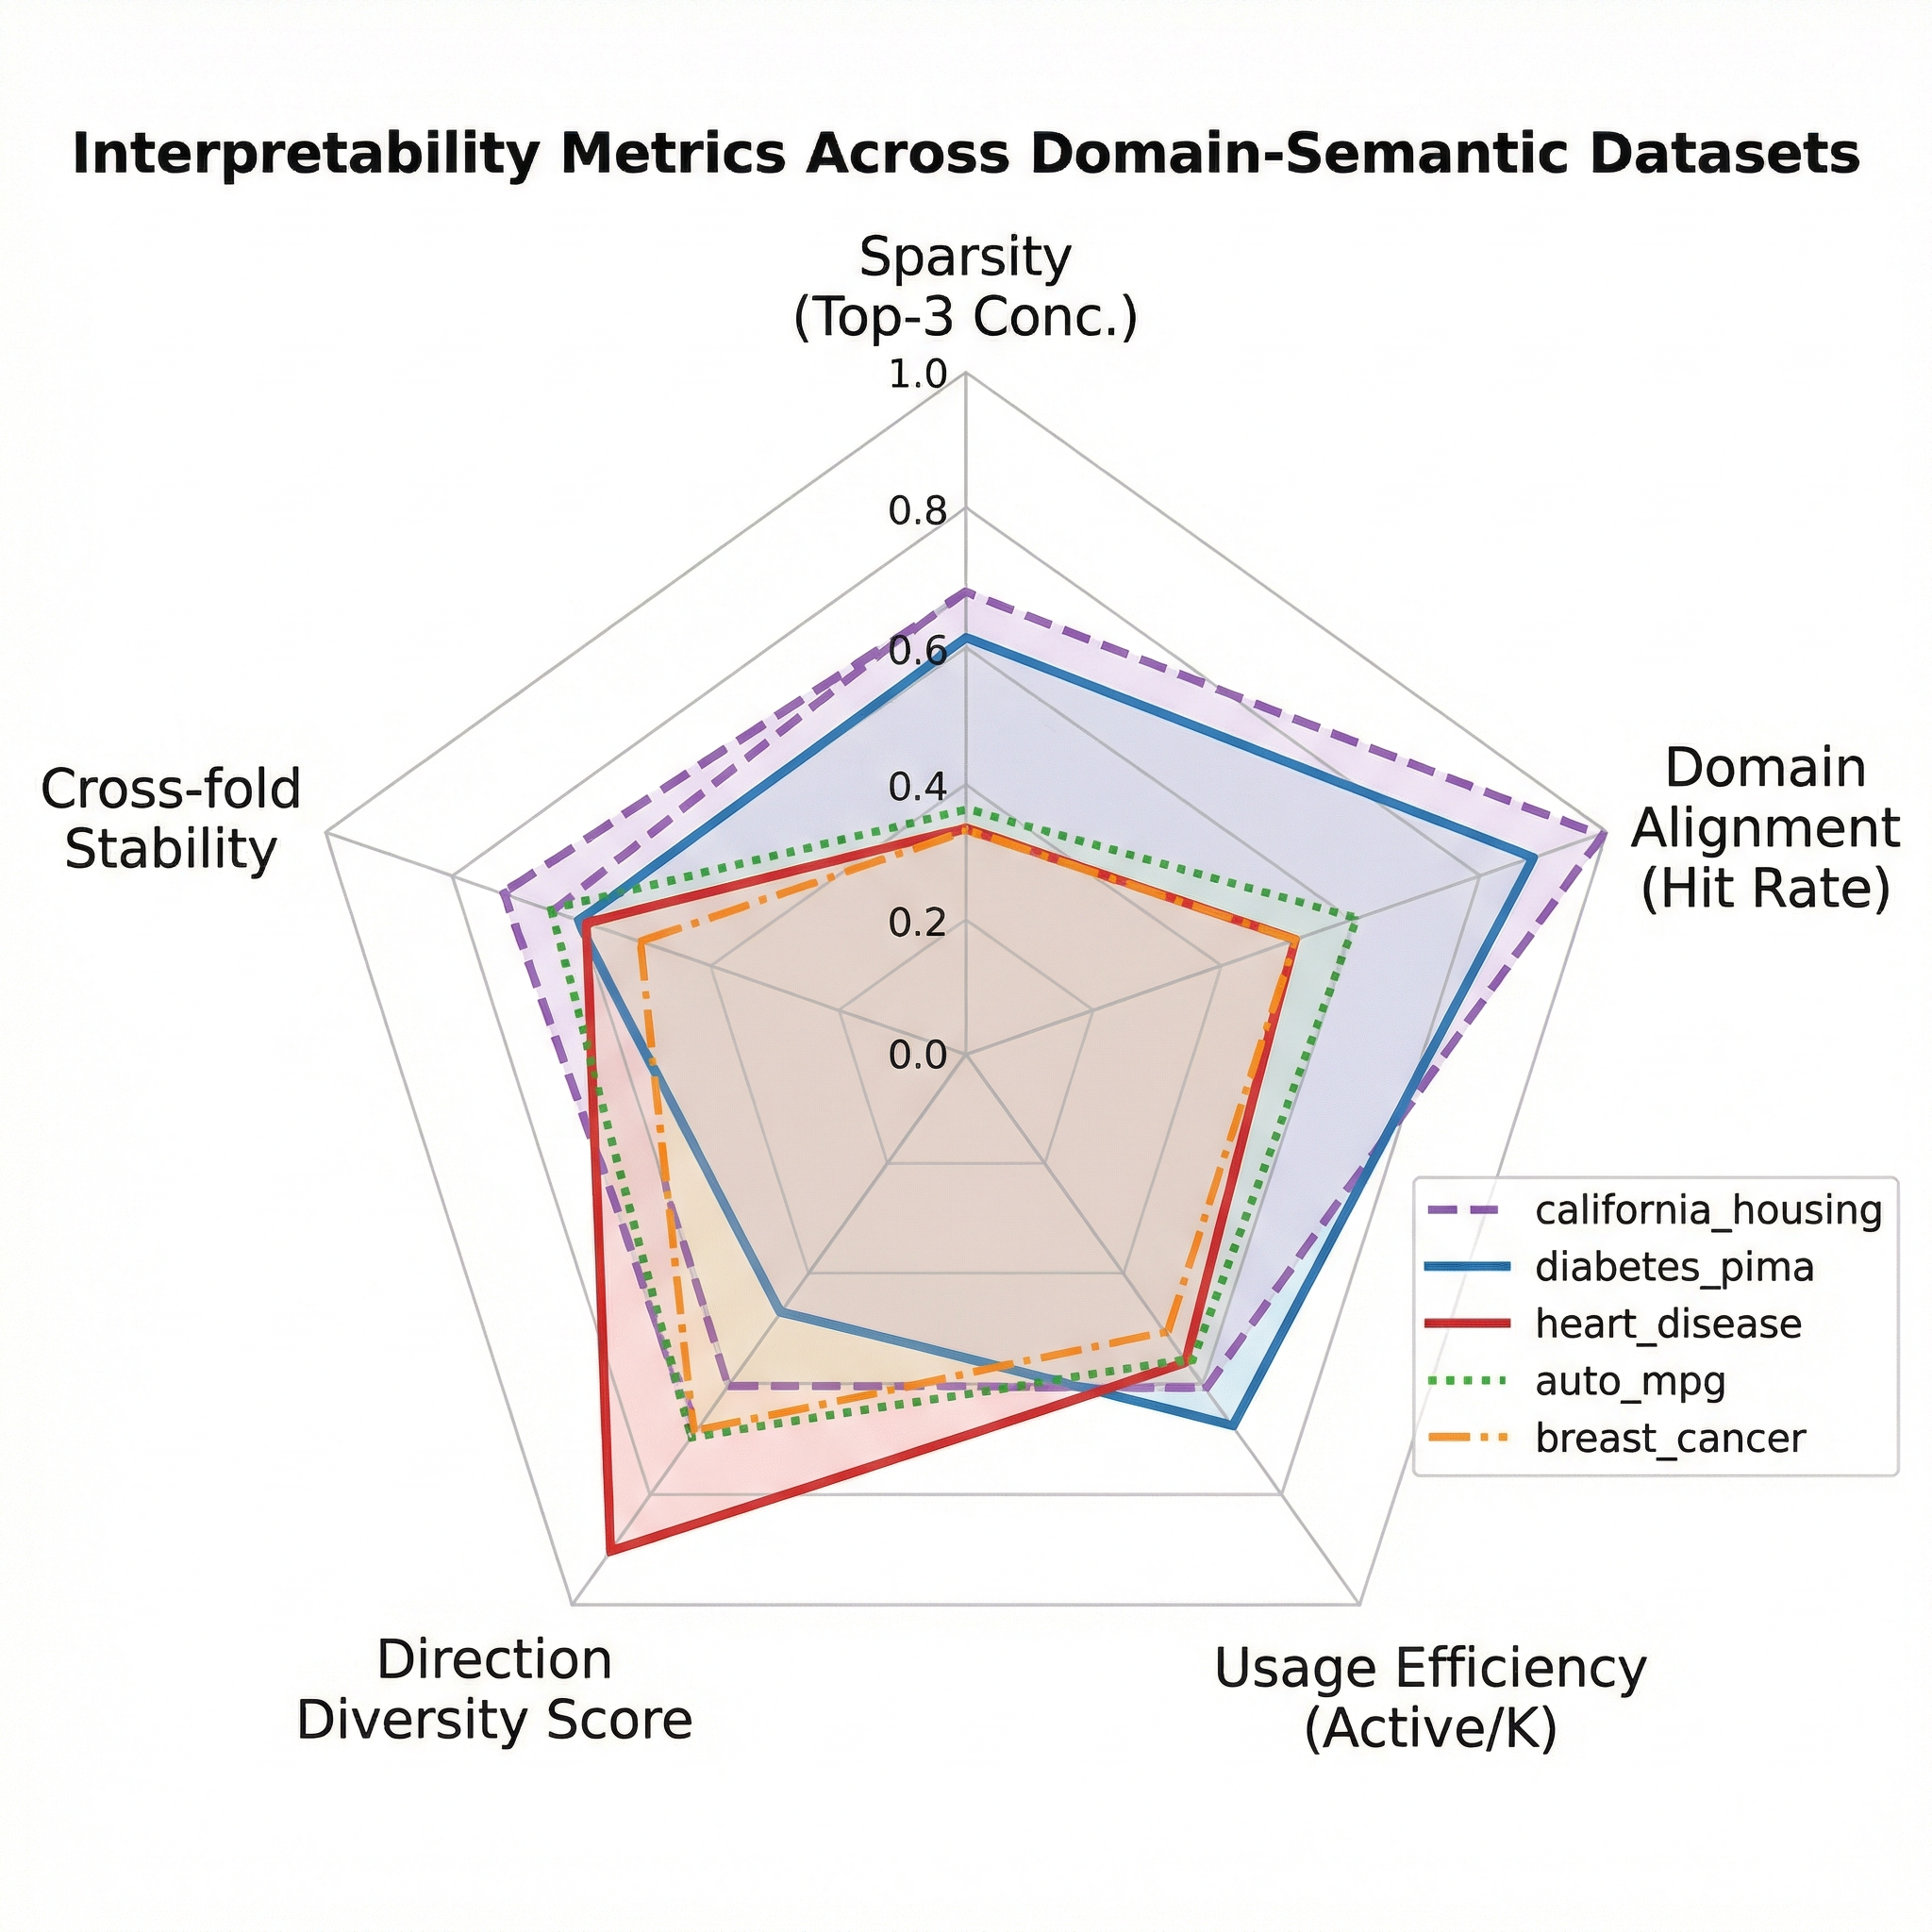
\includegraphics[width=0.70\textwidth,max height=0.40\textheight]{figures/fig_4_v0.png}
  \caption{Radar chart of interpretability metrics across five domain-semantic datasets. California\_housing and diabetes\_pima achieve the highest sparsity and domain alignment, while heart\_disease shows the highest direction diversity but lower domain alignment.}
  \label{fig:interpretability_radar}
\end{figure}

\subsection{Ablation Study}

A systematic ablation of 3 initialization strategies (PCA, Random, LDA) $\times$ 2 refinement strategies (WLS, L-BFGS) at $K = 8$ with 5 alternation rounds revealed:

\textbf{Initialization.} Random initialization achieves the best mean rank (2.1 across configurations), followed by LDA (2.5) and PCA (3.2). This counterintuitive result suggests that principal components of the feature matrix are not necessarily aligned with optimal decision boundaries, and the alternating optimization can recover good directions from arbitrary starting points.

\textbf{Refinement.} WLS refinement consistently outperforms L-BFGS on average, likely because the closed-form solution is more stable than iterative gradient optimization in the alternating framework.

\textbf{Iteration improvement.} The mean improvement from initial to refined implementation was 11.35 percentage points, underscoring that algorithmic engineering quality dominates the codebook concept itself.

% ============================================================
% 6. DISCUSSION
% ============================================================
\section{Discussion}

\subsection{The Codebook Constraint is Free}

The central finding of this work is that constraining all oblique splits to select from a small shared codebook does not significantly harm accuracy. The gap decomposition establishes this rigorously: Gap~B $= -0.031$ with $p = 0.43$ is not statistically significant, with the 95\% confidence interval $[-0.079, +0.007]$ straddling zero and the negative point estimate suggesting a mild \emph{benefit} from the codebook constraint---consistent with the hypothesis that the codebook acts as beneficial regularization analogous to weight-tying in neural networks.

This finding validates the core premise that real-world tabular data contains redundant structure: decision boundaries cluster around a modest number of canonical directions in feature space, far fewer than the total number of splits. The per-dataset optimal $K$ values ($K = 3$ for 6/10 datasets) and the active codebook sizes (mean 3.52 out of 8) provide converging evidence for this claim.

\subsection{Comparison with Prior Work}

Codebook-FIGS occupies a unique position in the interpretability-performance landscape. Unlike SPORF~\citep{Tomita2020}, which uses random projections with no learned shared structure, Codebook-FIGS learns a compact set of reusable directions. Unlike RO-FIGS~\citep{Mattikalli2025}, which independently optimizes each node's direction, Codebook-FIGS enforces global coherence through the shared codebook. Unlike SREDT~\citep{Fong2024} and FoLDTree~\citep{Wang2024}, which increase per-node expressiveness, Codebook-FIGS deliberately constrains it in exchange for ensemble-level interpretability.

The conceptual parallel to sparse autoencoders~\citep{Cunningham2024} is striking: just as SAEs discovered that neural network activations decompose into sparse combinations of a shared feature dictionary, Codebook-FIGS shows that tree ensemble decision boundaries can be expressed through a shared direction dictionary. The key difference is that in tree ensembles, each split selects exactly one dictionary atom (hard assignment) rather than a sparse linear combination (soft assignment).

\begin{figure}[!htbp]
  \centering
  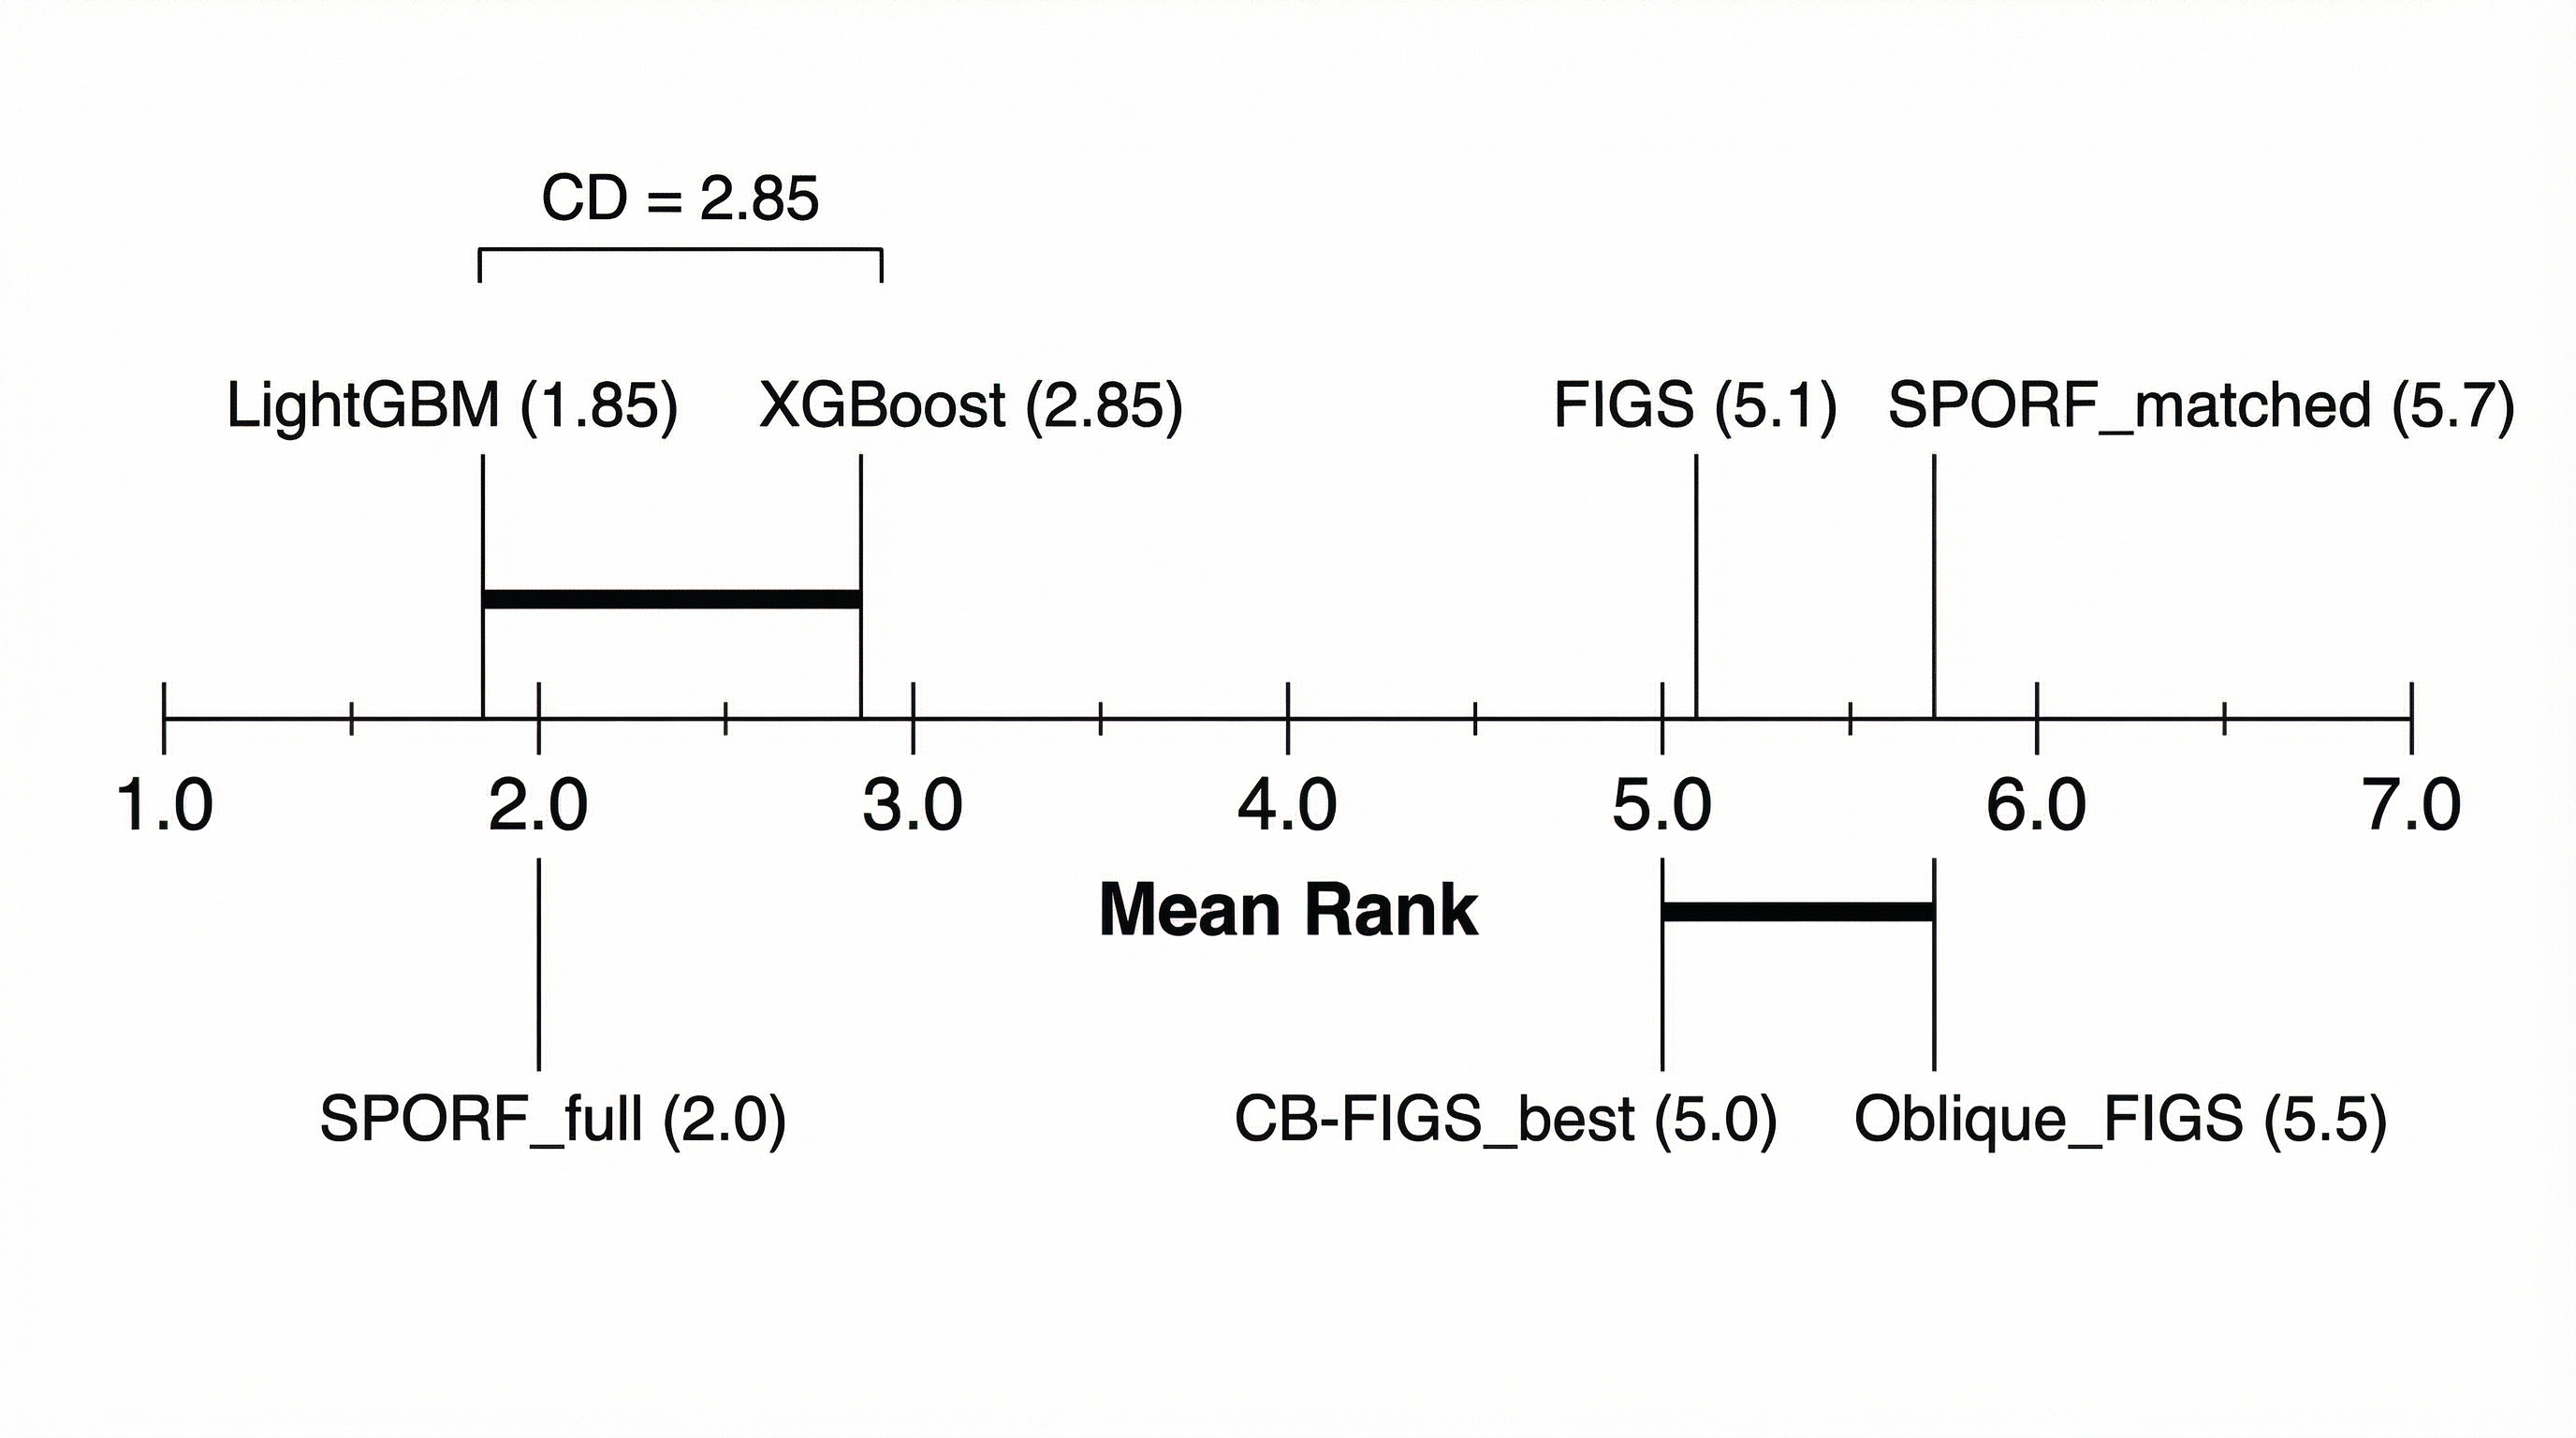
\includegraphics[width=0.85\textwidth,max height=0.30\textheight]{figures/fig_5_v0.png}
  \caption{Friedman-Nemenyi critical difference diagram. Methods connected by a horizontal bar are not significantly different (CD $= 2.85$). CB-FIGS (rank 5.0) is statistically indistinguishable from FIGS (5.1) but significantly worse than LightGBM (1.85) and SPORF-full (2.0).}
  \label{fig:cd_diagram}
\end{figure}

\subsection{Limitations}

\textbf{Codebook stability.} Mean cosine similarity of 0.554 across CV folds falls well below the 0.80 target. This may reflect a fundamental identifiability issue---multiple equally valid codebooks may achieve similar performance---or insufficient regularization. The v2 algorithm with elastic-net sparsity achieved 0.835 on isolated folds, suggesting the target is achievable with further optimization improvements.

\textbf{Codebook sparsity.} Mean top-3 feature concentration of 0.414 and Gini coefficient of 0.378 indicate that codebook directions are not yet sparse enough for the ``named direction'' interpretability vision (e.g., ``metabolic risk $= 0.6 \times \text{BMI} + 0.3 \times \text{glucose} + 0.1 \times \text{age}$''). Stronger sparsity-inducing penalties or post-hoc sparsification may be needed.

\textbf{Gap with gradient-boosted ensembles.} Codebook-FIGS (rank 5.0) trails XGBoost (2.85) and LightGBM (1.85) substantially. This gap is shared with axis-aligned FIGS (rank 5.1) and reflects the inherent accuracy cost of compact, interpretable models relative to large black-box ensembles---not a codebook-specific limitation.

\textbf{California housing and wine quality.} These regression datasets show the largest gaps (23.3pp and 9.6pp vs.\ FIGS), potentially because their complex, high-dimensional decision surfaces require more than $K = 8$ directions or because the alternating optimization struggles with larger sample sizes (california\_housing has 20,640 samples).

\textbf{No domain expert evaluation.} Our ``domain alignment'' metric is automated. No cardiologists, endocrinologists, or other domain experts evaluated whether the codebook directions correspond to genuinely meaningful clinical or scientific concepts.

% ============================================================
% 7. CONCLUSION
% ============================================================
\section{Conclusion}

We introduced Codebook-FIGS, the first tree ensemble method that constrains all oblique splits to select from a small, jointly learned dictionary of shared directions. Through a rigorous diagnostic gap decomposition, we established that the codebook constraint is statistically free (Gap~B $= -0.031$, $p = 0.43$)---the performance bottleneck lies in oblique split optimization quality, not the codebook concept. Small codebooks of $K = 3$--$5$ suffice for most datasets, with clear elbows in 80\% of benchmarks, confirming that tabular decision boundaries cluster around a few canonical directions. Codebook-FIGS achieves parity with axis-aligned FIGS (rank 5.0 vs.\ 5.1) while compressing direction diversity by $2.1\times$.

This work opens several directions for future research. First, improving oblique split optimization (closing Gap~A $= +0.060$) would directly benefit Codebook-FIGS, potentially placing it above axis-aligned FIGS. Second, stronger sparsity-inducing penalties or post-hoc sparsification could enable the ``named direction'' interpretability vision. Third, gradient-based end-to-end codebook learning (rather than alternating minimization) could improve both accuracy and codebook stability. Finally, the codebook paradigm could extend beyond FIGS to gradient-boosted ensembles and random forests, potentially bringing dictionary-learning-based interpretability to the most widely used tree ensemble methods.

% ============================================================
% REFERENCES
% ============================================================
\bibliographystyle{plainnat}
\bibliography{references}

\end{document}
